% +------------------------------------------------------------------------+
% | Reference manual page: Subdivision_surfaces_3.tex
% +------------------------------------------------------------------------+
% | 03/01/2005   Le-Jeng Andy Shiue
% | Package: Subdivision_surface_3
% | 
\RCSdef{\RCSSubdivisionRev}{$Revision$}
\RCSdefDate{\RCSSubdivisionDate}{$Date$}
% +------------------------------------------------------------------------+

\ccRefPageBegin

%%RefPage: end of header, begin of main body
% +------------------------------------------------------------------------+


\begin{ccRefClass}{PQQ_stencil}

\ccDefinition

Stencils define the mapping from a submesh of the control mesh to a 
point on the refined mesh. \ccClassTemplateName , used as the base 
class of the geometry stencils, consists of three stencils of the 
PQQ refinement. \ccClassTemplateName\ can also be used to define 
the interface of PTQ and Sqrt(3) stencils.


%% \begin{ccTexOnly}
%%     \vspace{-7mm}
%%     \begin{center}
%%       \parbox{0.4\textwidth}{%
%%         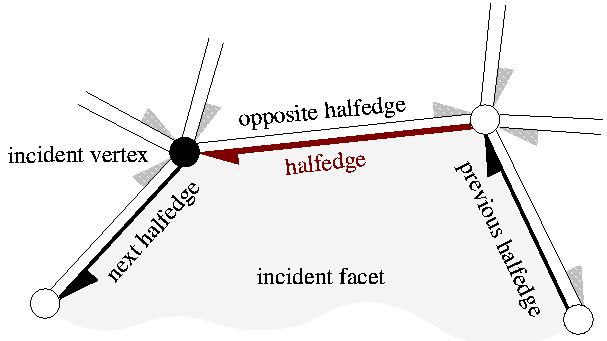
\includegraphics[width=0.4\textwidth]{Polyhedron_ref/fig/halfedge}%
%%       }
%%     \end{center}
%%     \vspace{-5mm}
%% \end{ccTexOnly}

%% \begin{ccHtmlOnly}
%%     <CENTER>
%%     <A HREF="fig/halfedge.gif">
%%         <img src="fig/halfedge_small.gif" alt="Halfedge Diagram"></A><P>
%%     </CENTER>
%% \end{ccHtmlOnly}

\ccInclude{CGAL/Subdivision_surfaces_rules_3.h}

\ccParameters

The full template declaration of \ccClassTemplateName\ states one
template parameter:

\begin{tabbing}
\ccc{template <} \=\ccc{class _Poly>}\\
     \ccc{class PQQ_stencil;}
\end{tabbing}
   
The \ccc{_Poly} parameter requires requires a model of 
the \ccc{Polyhedron_3} concept as argument. \ccc{Point_3} 
type is reqiured to be defined in the \ccc{_Poly}.

%% \ccTypes

%% \ccNestedType{Traits}{traits class selected for \ccc{PolyhedronTraits_3}.}
%% \ccGlue
%% \ccNestedType{Items}{items class selected for \ccc{PolyhedronItems_3}.}
%% \ccGlue



%% % +-----------------------------------+
%% \begin{ccAdvanced}
%% \ccHeading{Types for Tagging Optional Features}

%% \ccNestedType{Supports_facet_plane}{\ccc{Facet::plane()}.}
%% \ccGlue
%% \ccNestedType{Supports_removal}{supports removal of individual elements.}

%% \end{ccAdvanced}

\ccCreation
%\ccCreationVariable{P}

\ccClassTemplateName\ is a functor of the three geometry stencils for
subdivision surfaces based on the PQQ refinement. Default constructor 
is generated by the compiler.


% +-----------------------------------+
\ccHeading{Stencil Policies}
\ccThree{}{}{}

\ccMethod{void facet_node(Facet_handle f, Point& pt)}
{an empty function defining the interface of the facet-node stencil 
of the PQQ refinement.}

\ccMethod{void edge_node(Edge_handle e, Point& pt)}
{an empty function defining the interface of the edge-node stencil 
of the PQQ refinement.}

\ccMethod{void vertex_node(Vertex_handle v, Point& pt)}
{an empty function defining the interface of the vertex-node stencil
of the PQQ refinement.}

%% \begin{ccTexOnly}
%%     \begin{center}
%%       \parbox{0.636\textwidth}{%
%%           \includegraphics[width=0.636\textwidth]%
%%               {Polyhedron_ref/fig/euler_loop}%
%%       }
%%     \end{center}
%% \end{ccTexOnly}
%% \begin{ccHtmlOnly}
%%     <CENTER>
%%     <img src="fig/euler_loop.gif" alt="Euler Operator: Loop"><P>
%%     </CENTER>
%% \end{ccHtmlOnly}


\ccSeeAlso

\ccRefIdfierPage{CGAL::Subdivision_surfaces_3}\\

\ccExample

This example program instantiates a polyhedron using the default
traits class and creates a tetrahedron.

%\ccIncludeExampleCode{Polyhedron/polyhedron_prog_simple.C}

\end{ccRefClass}

% +------------------------------------------------------------------------+
%%RefPage: end of main body, begin of footer
\ccRefPageEnd
% EOF
% +------------------------------------------------------------------------+
\ccRefPageBegin

%%RefPage: end of header, begin of main body
% +------------------------------------------------------------------------+




% +------------------------------------------------------------------------+
% +------------------------------------------------------------------------+
\begin{ccRefClass}{DQQ_stencil}

\ccDefinition

Stencils define the mapping from a submesh of the control mesh to a 
point on the refined mesh. \ccClassTemplateName , used as the base 
class of the geometry stencils, declares the corner-node
stencil of the DQQ refinement. 

\ccInclude{CGAL/Subdivision_surfaces_rules_3.h}

\ccParameters

The full template declaration of \ccClassTemplateName\ states one
template parameter:

\begin{tabbing}
\ccc{template <} \=\ccc{class _Poly>}\\
     \ccc{class DQQ_stencil;}
\end{tabbing}
   
The \ccc{_Poly} parameter requires requires a model of 
the \ccc{Polyhedron_3} concept as argument. \ccc{Point_3} 
type is reqiured to be defined in the \ccc{_Poly}.

\ccCreation
%\ccCreationVariable{P}

\ccClassTemplateName\ is a functor of the three geometry stencils for
subdivision surfaces based on the PQQ refinement. Default constructor 
is generated by the compiler.


% +-----------------------------------+
\ccHeading{Stencil Policies}
\ccThree{}{}{}

\ccMethod{void corner_node(Halfedge_handle edge, Point& pt)}
{an empty function defining the interface of the corner-node stencil 
of the DQQ refinement. \ccc{edge} points to the vertex that has 
dominate weight to smooth \ccc{pt}.}

\ccSeeAlso

\ccRefIdfierPage{CGAL::Subdivision_surfaces_3}\\

\end{ccRefClass}

% +------------------------------------------------------------------------+
%%RefPage: end of main body, begin of footer
\ccRefPageEnd
% EOF
% +------------------------------------------------------------------------+



% +------------------------------------------------------------------------+
% +------------------------------------------------------------------------+
\begin{ccRefClass}{Linear_stencil}

\ccDefinition

Stencils define the mapping from a submesh of the control mesh to a 
point on the refined mesh. \ccClassTemplateName , derived from 
\ccc{PQQ_stencil}, defines the geometry stencils as linear 
averaging of the points collected from the submesh of the 
control mesh.

\ccInclude{CGAL/Subdivision_surfaces_rules_3.h}

\ccParameters

The full template declaration of \ccClassTemplateName\ states one
template parameter:

\begin{tabbing}
\ccc{template <} \=\ccc{class _Poly>}\\
     \ccc{class Linear_stencil;}
\end{tabbing}
   
The \ccc{_Poly} parameter requires requires a model of 
the \ccc{Polyhedron_3} concept as argument. \ccc{Point_3} 
type is reqiured to be defined in the \ccc{_Poly}.

\ccCreation
%\ccCreationVariable{P}

Default constructor is generated for \ccClassTemplateName\ by the compiler.


% +-----------------------------------+
\ccHeading{Stencil Policies}
\ccThree{}{}{}

\ccMethod{void facet_node(Facet_handle f, Point& pt)}
{assign the linear average of the points on \ccc{f} to \ccc{pt}}

\ccMethod{void edge_node(Edge_handle e, Point& pt)}
{assign the linear average of the points on \ccc{e} to \ccc{pt}}

\ccMethod{void vertex_node(Vertex_handle v, Point& pt)}
{assign the point on \ccc{v} to \ccc{pt}}

\ccSeeAlso

\ccRefIdfierPage{CGAL::Subdivision_surfaces_3}\\

\end{ccRefClass}

% +------------------------------------------------------------------------+
%%RefPage: end of main body, begin of footer
\ccRefPageEnd
% EOF
% +------------------------------------------------------------------------+



% +------------------------------------------------------------------------+
% +------------------------------------------------------------------------+
\begin{ccRefClass}{CatmullClark_stencil}

\ccDefinition

\ccClassTemplateName\ defines the 
geometry stencils of Catmull-Clark subdivision. 

\ccInclude{CGAL/Subdivision_surfaces_rules_3.h}

\ccParameters

The full template declaration of \ccClassTemplateName\ states one
template parameter:

\begin{tabbing}
\ccc{template <} \=\ccc{class _Poly>}\\
     \ccc{class Linear_stencil;}
\end{tabbing}
   
The \ccc{_Poly} parameter requires requires a model of 
the \ccc{Polyhedron_3} concept as argument. \ccc{Point_3} 
type is reqiured to be defined in the \ccc{_Poly}.

\ccCreation
%\ccCreationVariable{P}

Default constructor is generated for \ccClassTemplateName\ by the compiler.

% +-----------------------------------+
\ccHeading{Stencil Policies}
\ccThree{}{}{}

\ccMethod{void facet_node(Facet_handle f, Point& pt)}
{caculate the facet point of Catmull-Clark subdivision based on \ccc{f}, 
and assign the smoothed point to \ccc{pt}.}

\ccMethod{void edge_node(Edge_handle e, Point& pt)}
{caculate the edge point of Catmull-Clark subdivision based on the 1-ring
of \ccc{e}, and assign the smoothed point to \ccc{pt}.}

\ccMethod{void vertex_node(Vertex_handle v, Point& pt)}
{caculate the vertex point of Catmull-Clark subdivision based on the 
1-ring of \ccc{v}, and assign the smoothed point to \ccc{pt}.}


\ccSeeAlso

\ccRefIdfierPage{CGAL::Subdivision_surfaces_3}\\

\end{ccRefClass}

% +------------------------------------------------------------------------+
%%RefPage: end of main body, begin of footer
\ccRefPageEnd
% EOF
% +------------------------------------------------------------------------+


% +------------------------------------------------------------------------+
% +------------------------------------------------------------------------+
\begin{ccRefClass}{Loop_stencil}

\ccDefinition

\ccClassTemplateName\ defines the 
geometry stencils of Loop subdivision. 

\ccInclude{CGAL/Subdivision_surfaces_rules_3.h}

\ccParameters

The full template declaration of \ccClassTemplateName\ states one
template parameter:

\begin{tabbing}
\ccc{template <} \=\ccc{class _Poly>}\\
     \ccc{class Linear_stencil;}
\end{tabbing}
   
The \ccc{_Poly} parameter requires requires a model of 
the \ccc{Polyhedron_3} concept as argument. \ccc{Point_3} 
type is reqiured to be defined in the \ccc{_Poly}.

\ccCreation
%\ccCreationVariable{P}

Default constructor is generated for \ccClassTemplateName\ by the compiler.

% +-----------------------------------+
\ccHeading{Stencil Policies}
\ccThree{}{}{}

\ccMethod{void edge_node(Edge_handle e, Point& pt)}
{caculate the edge point of Loop subdivision based on the 1-ring
of \ccc{e}, and assign the smoothed point to \ccc{pt}.}

\ccMethod{void vertex_node(Vertex_handle v, Point& pt)}
{caculate the vertex point of Loop subdivision based on the 
1-ring of \ccc{v}, and assign the smoothed point to \ccc{pt}.}


\ccSeeAlso

\ccRefIdfierPage{CGAL::Subdivision_surfaces_3}\\

\end{ccRefClass}

% +------------------------------------------------------------------------+
%%RefPage: end of main body, begin of footer
\ccRefPageEnd
% EOF
% +------------------------------------------------------------------------+


% +------------------------------------------------------------------------+
% +------------------------------------------------------------------------+
\begin{ccRefClass}{DooSabin_stencil}

\ccDefinition

\ccClassTemplateName\ defines the 
geometry stencils of Doo-Sabin subdivision. 

\ccInclude{CGAL/Subdivision_surfaces_rules_3.h}

\ccParameters

The full template declaration of \ccClassTemplateName\ states one
template parameter:

\begin{tabbing}
\ccc{template <} \=\ccc{class _Poly>}\\
     \ccc{class Linear_stencil;}
\end{tabbing}
   
The \ccc{_Poly} parameter requires requires a model of 
the \ccc{Polyhedron_3} concept as argument. \ccc{Point_3} 
type is reqiured to be defined in the \ccc{_Poly}.

\ccCreation
%\ccCreationVariable{P}

Default constructor is generated for \ccClassTemplateName\ by the compiler.

% +-----------------------------------+
\ccHeading{Stencil Policies}
\ccThree{}{}{}

\ccMethod{void corner_node(Halfedge_handle he, Point& pt)}
{caculate the smooth point of Doo-Sabin subdivision 
based on points on the facet of \ccc{he}, and assign the smoothed 
point to \ccc{pt}. \ccc{he} always points to the dominate vertex  
in the geometry stencil.}


\ccSeeAlso

\ccRefIdfierPage{CGAL::Subdivision_surfaces_3}\\

\end{ccRefClass}

% +------------------------------------------------------------------------+
%%RefPage: end of main body, begin of footer
\ccRefPageEnd
% EOF
% +------------------------------------------------------------------------+


% +------------------------------------------------------------------------+
% +------------------------------------------------------------------------+
\begin{ccRefClass}{Sqrt3_stencil}

\ccDefinition

\ccClassTemplateName\ defines the 
geometry stencils of Sqrt(3) subdivision. 

\ccInclude{CGAL/Subdivision_surfaces_rules_3.h}

\ccParameters

The full template declaration of \ccClassTemplateName\ states one
template parameter:

\begin{tabbing}
\ccc{template <} \=\ccc{class _Poly>}\\
     \ccc{class Linear_stencil;}
\end{tabbing}
   
The \ccc{_Poly} parameter requires requires a model of 
the \ccc{Polyhedron_3} concept as argument. \ccc{Point_3} 
type is reqiured to be defined in the \ccc{_Poly}.

\ccCreation
%\ccCreationVariable{P}

Default constructor is generated for \ccClassTemplateName\ by the compiler.

% +-----------------------------------+
\ccHeading{Stencil Policies}
\ccThree{}{}{}

\ccMethod{void facet_node(Facet_handle f, Point& pt)}
{caculate the centroid of \ccc{f}, and assign the centroid 
to \ccc{pt}.}

\ccMethod{void vertex_node(Vertex_handle v, Point& pt)}
{caculate the vertex point of Sqrt(3) subdivision based on the 
1-ring of \ccc{v}, and assign the smoothed point to \ccc{pt}.}


\ccSeeAlso

\ccRefIdfierPage{CGAL::Subdivision_surfaces_3}\\

\end{ccRefClass}

% +------------------------------------------------------------------------+
%%RefPage: end of main body, begin of footer
\ccRefPageEnd
% EOF
% +------------------------------------------------------------------------+

